\section{UML Diagrams}

\begin{figure}[p]
	%\centering
	%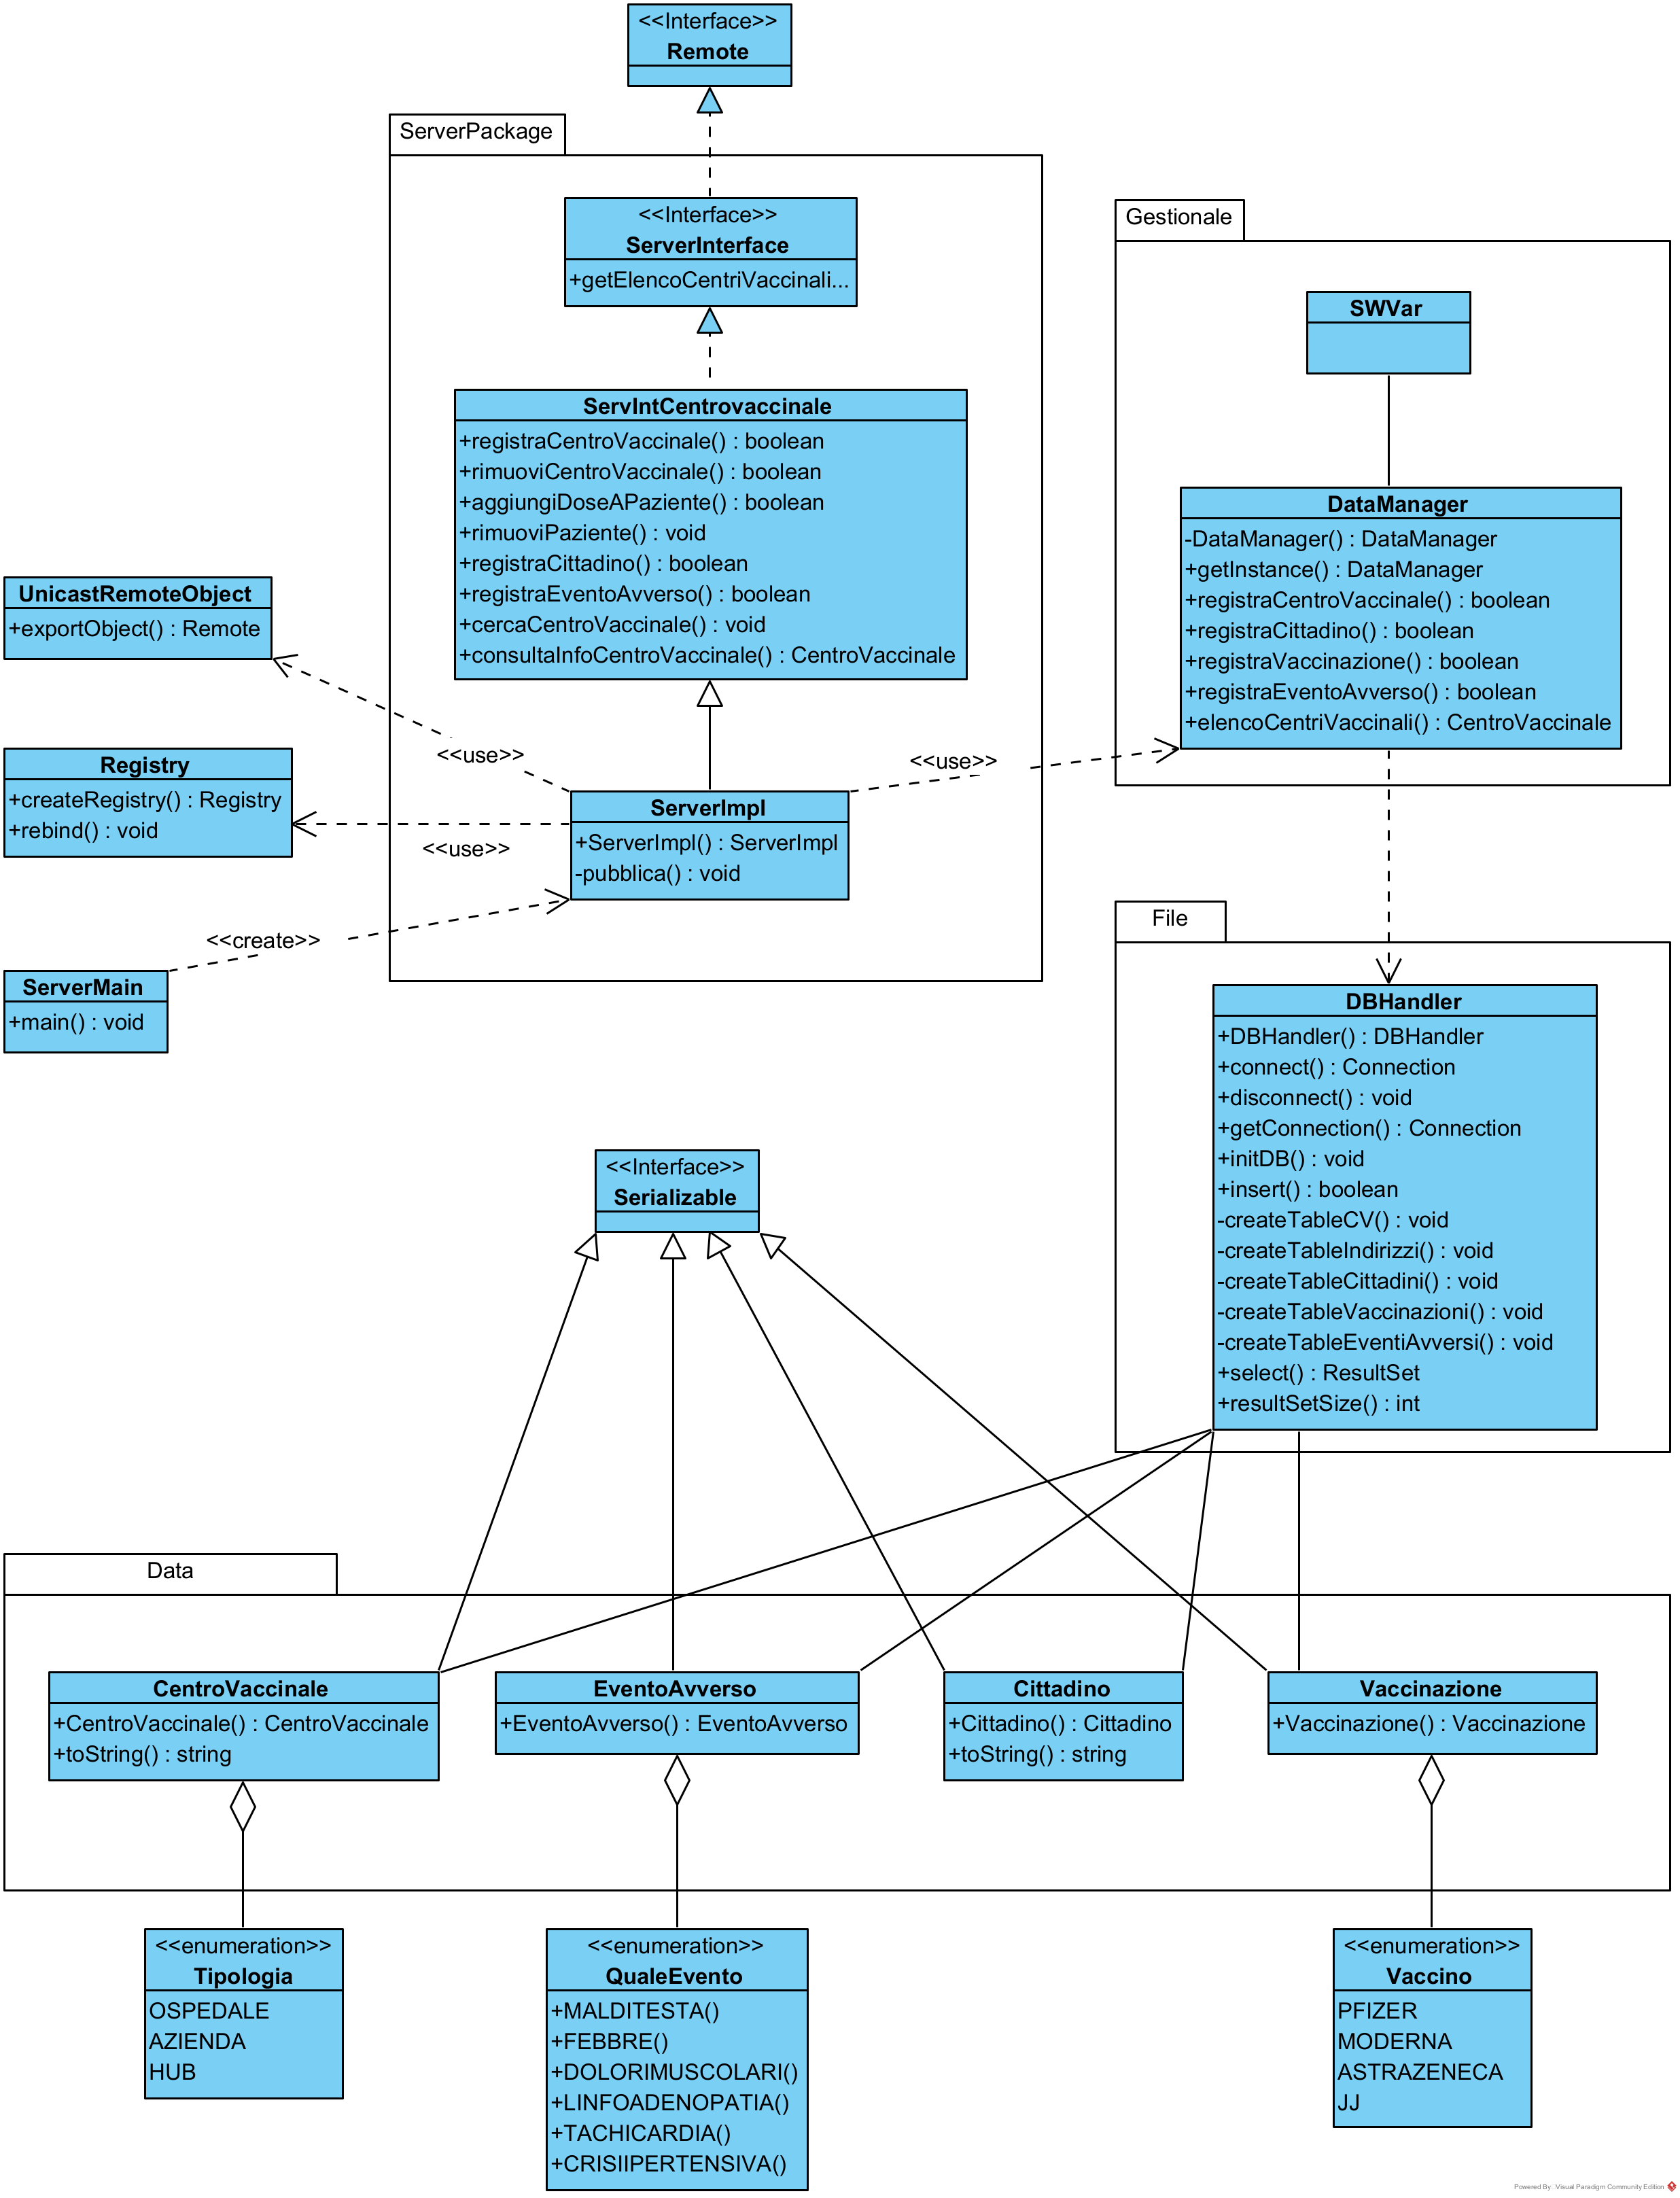
\includegraphics[width=\textwidth]{./img/Server}
	\makebox[\textwidth][c]{
		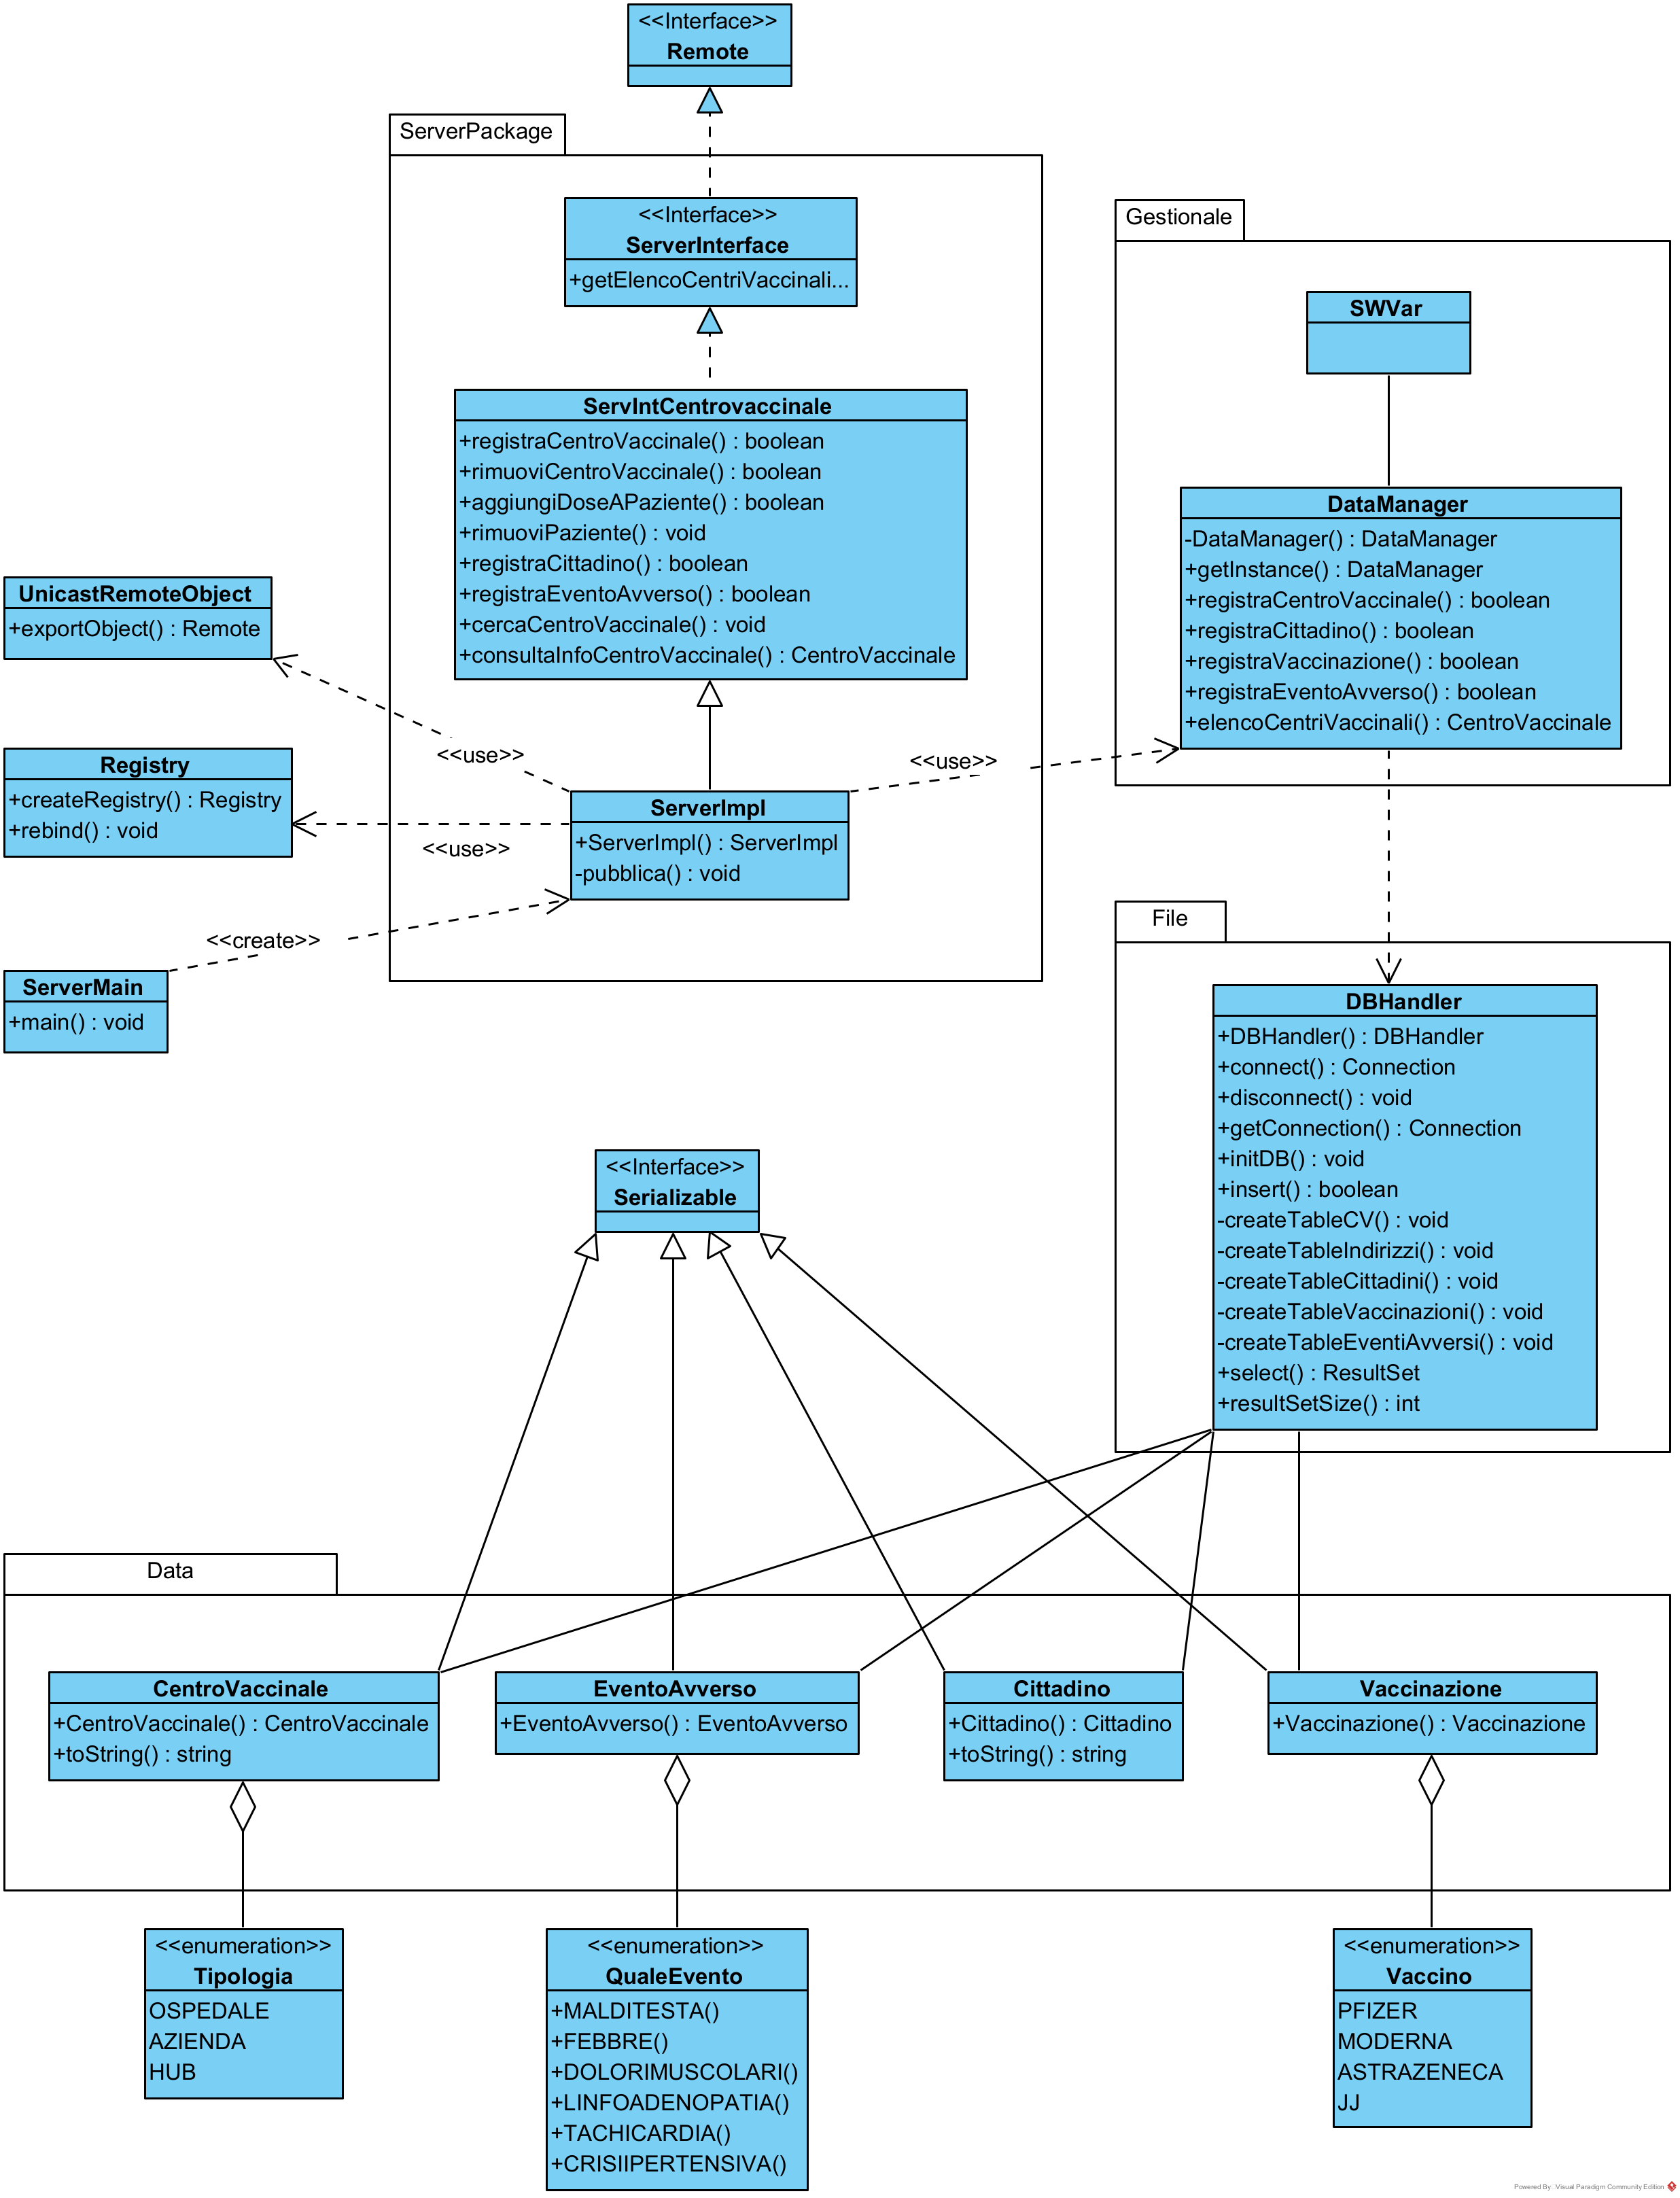
\includegraphics[width=1.3\textwidth]{./img/Server}
	}
	\caption{Class Diagram del modulo Server}
	\label{fig:classDiagramServer}
\end{figure}

\begin{figure}[t]
	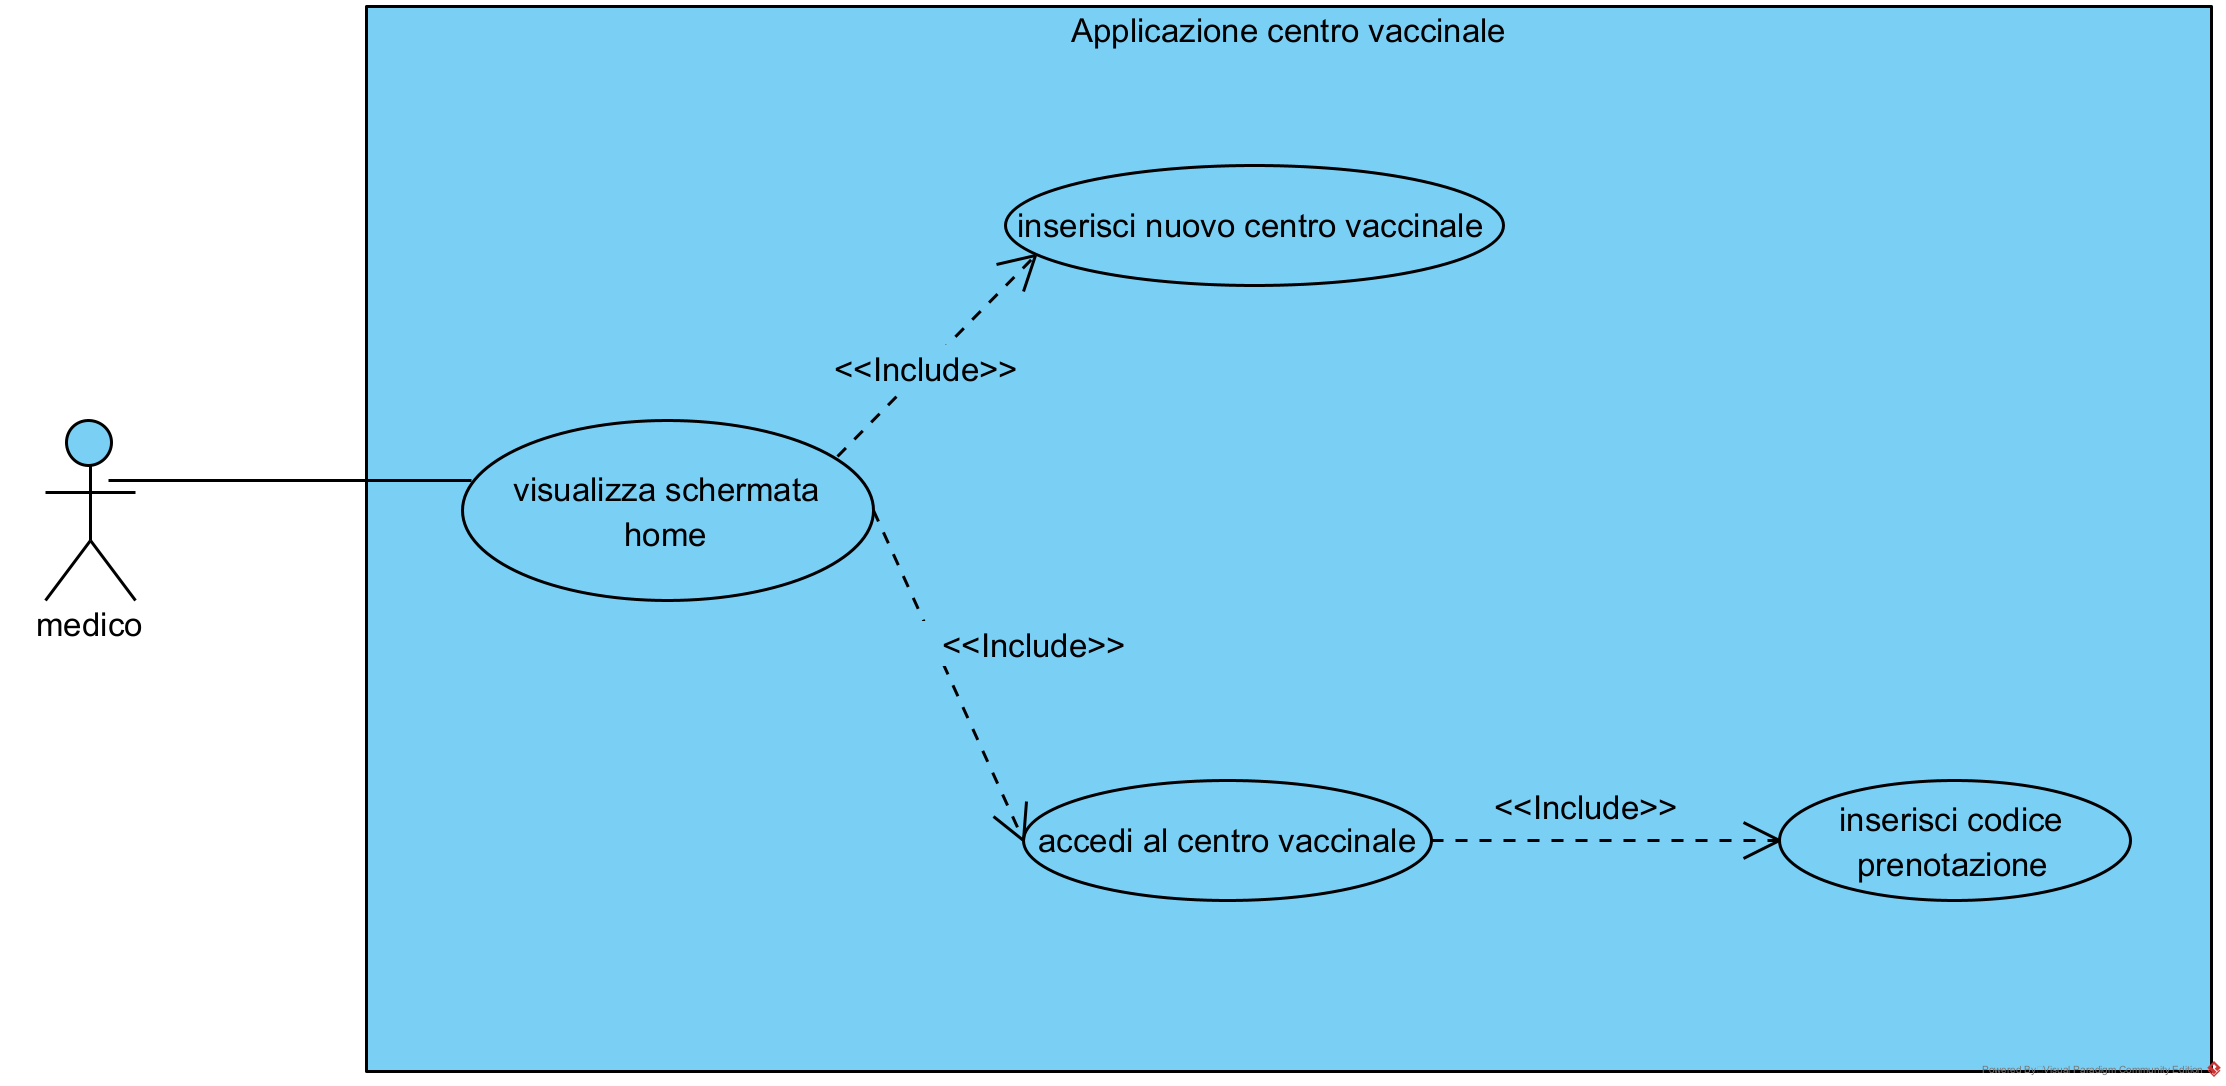
\includegraphics[width=\textwidth]{./img/UseCaseCentriVaccinali}
	\caption{Use case diagram del modulo centri vaccinali}
\end{figure}

\begin{figure}[t]
	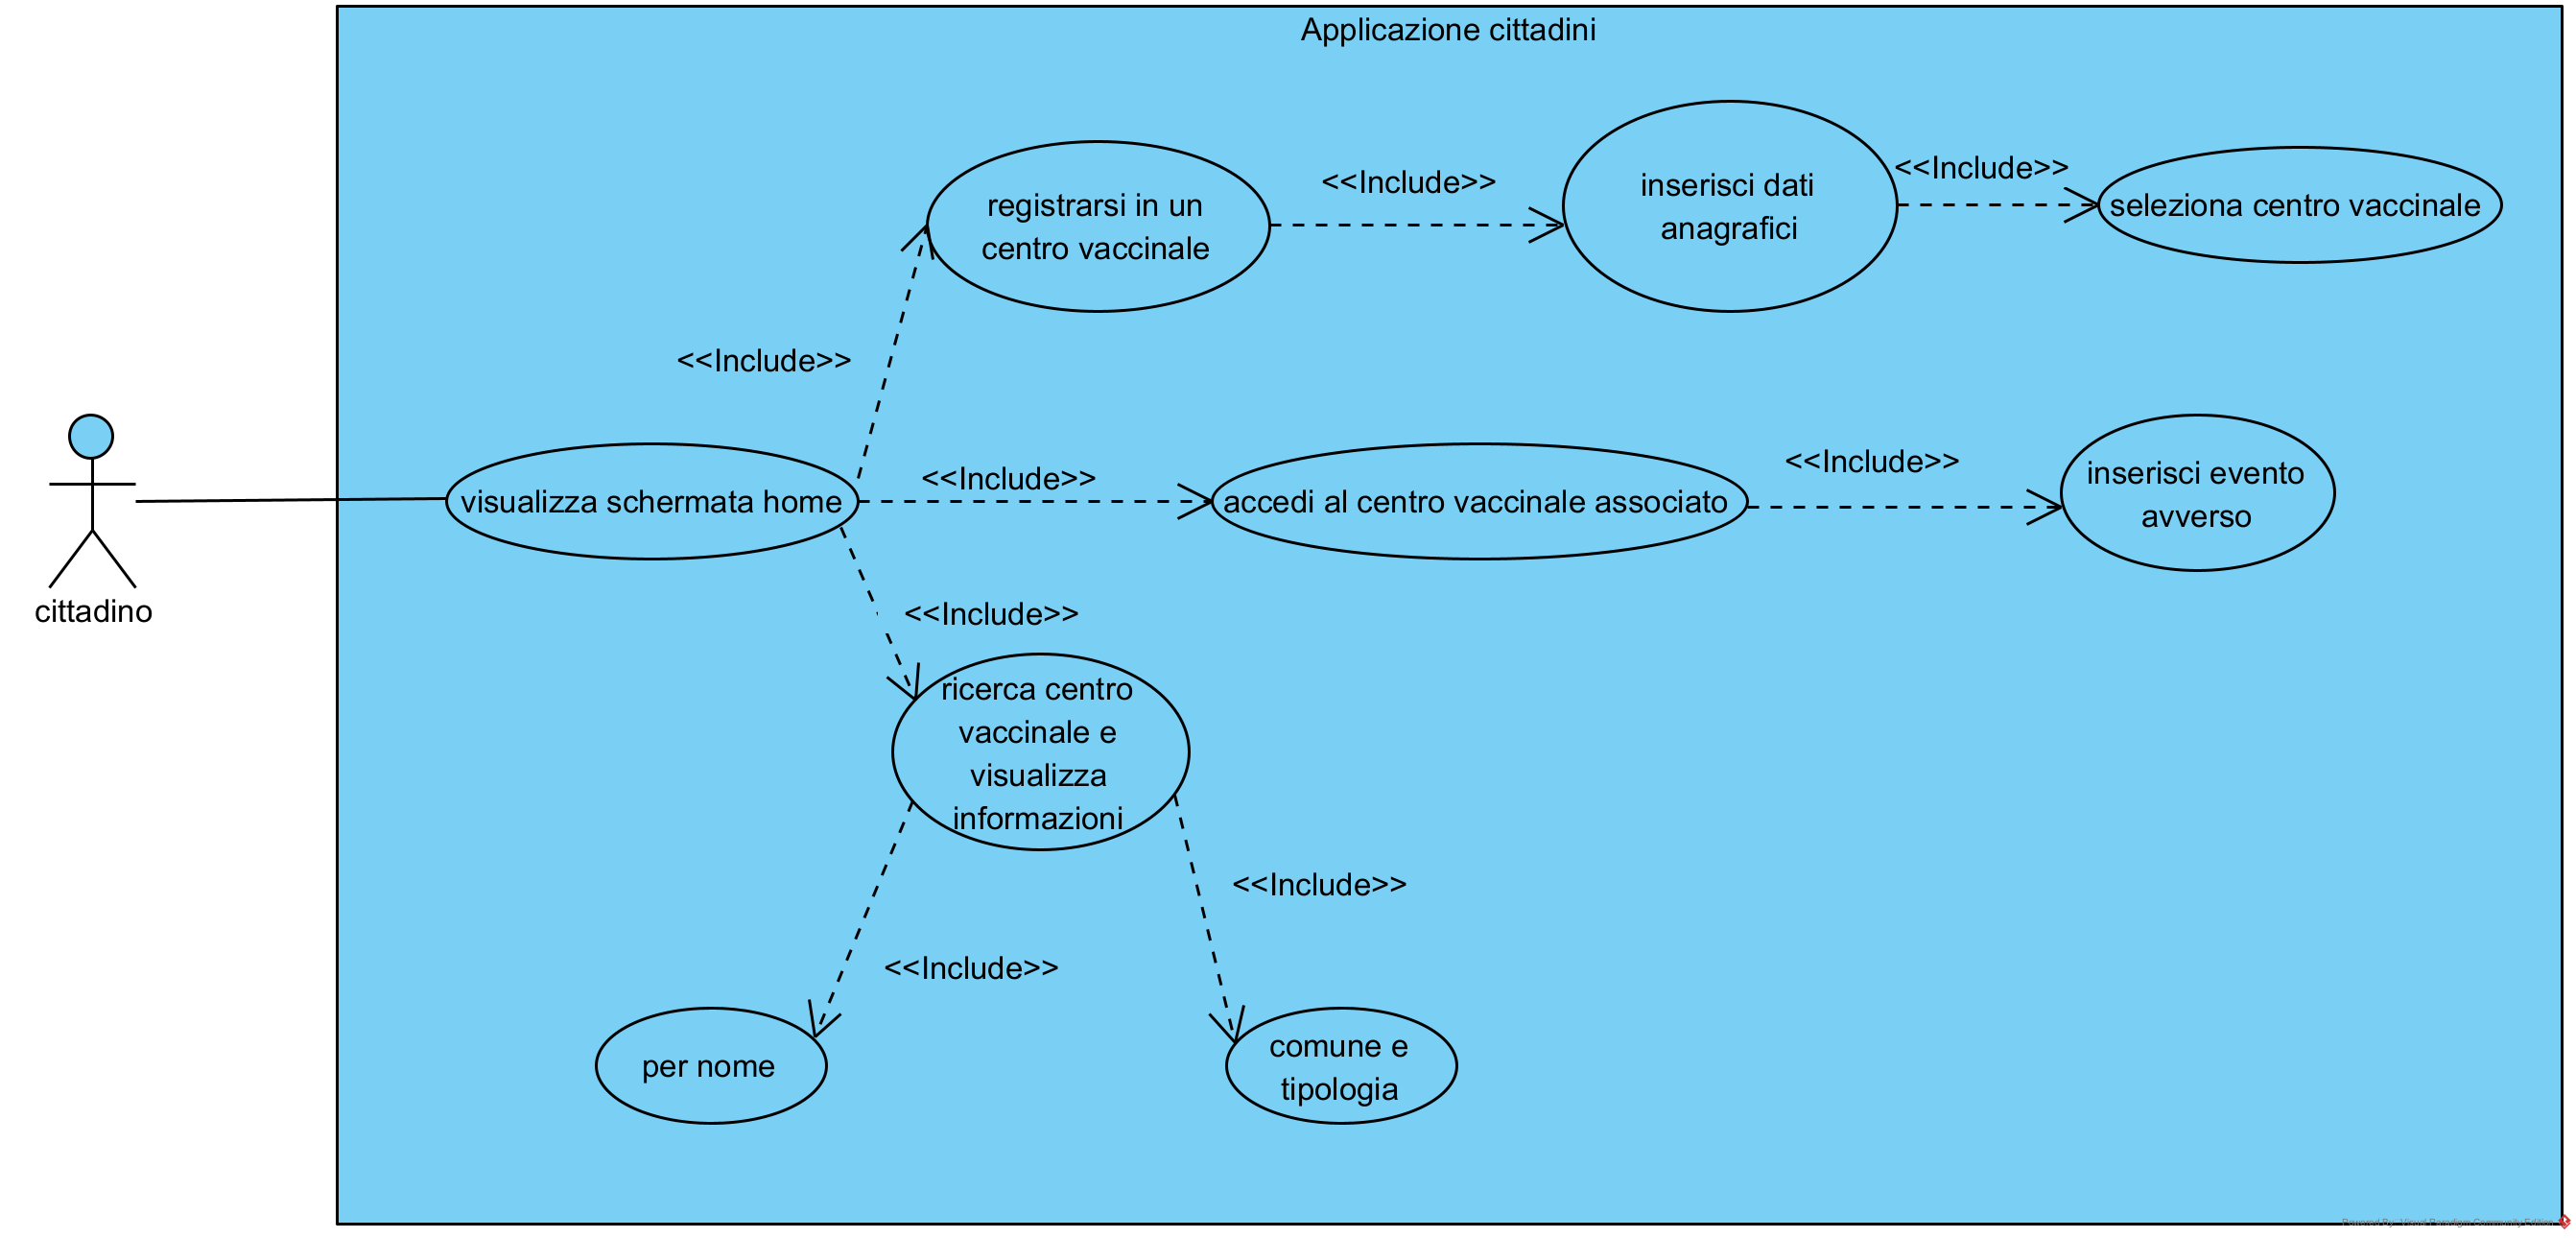
\includegraphics[width=\textwidth]{./img/UseCaseCittadino}
	\caption{Use case diagram del modulo cittadino}
\end{figure}

\begin{figure}[t]
	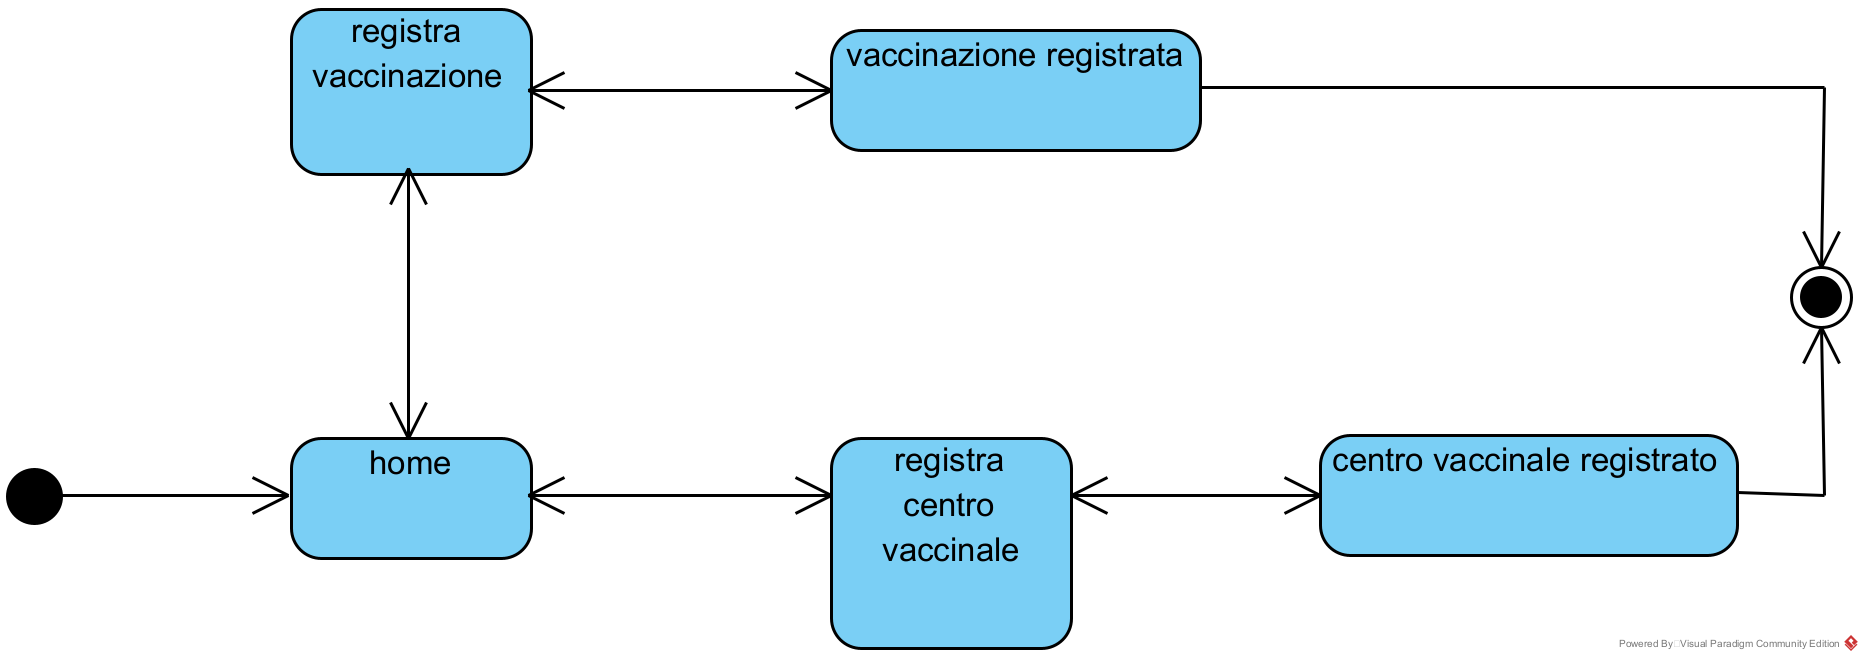
\includegraphics[width=\textwidth]{./img/StateMachineDiagramCentroVaccinale}
	\caption{State diagram del modulo centro vaccinale}
\end{figure}

\begin{figure}[t]
	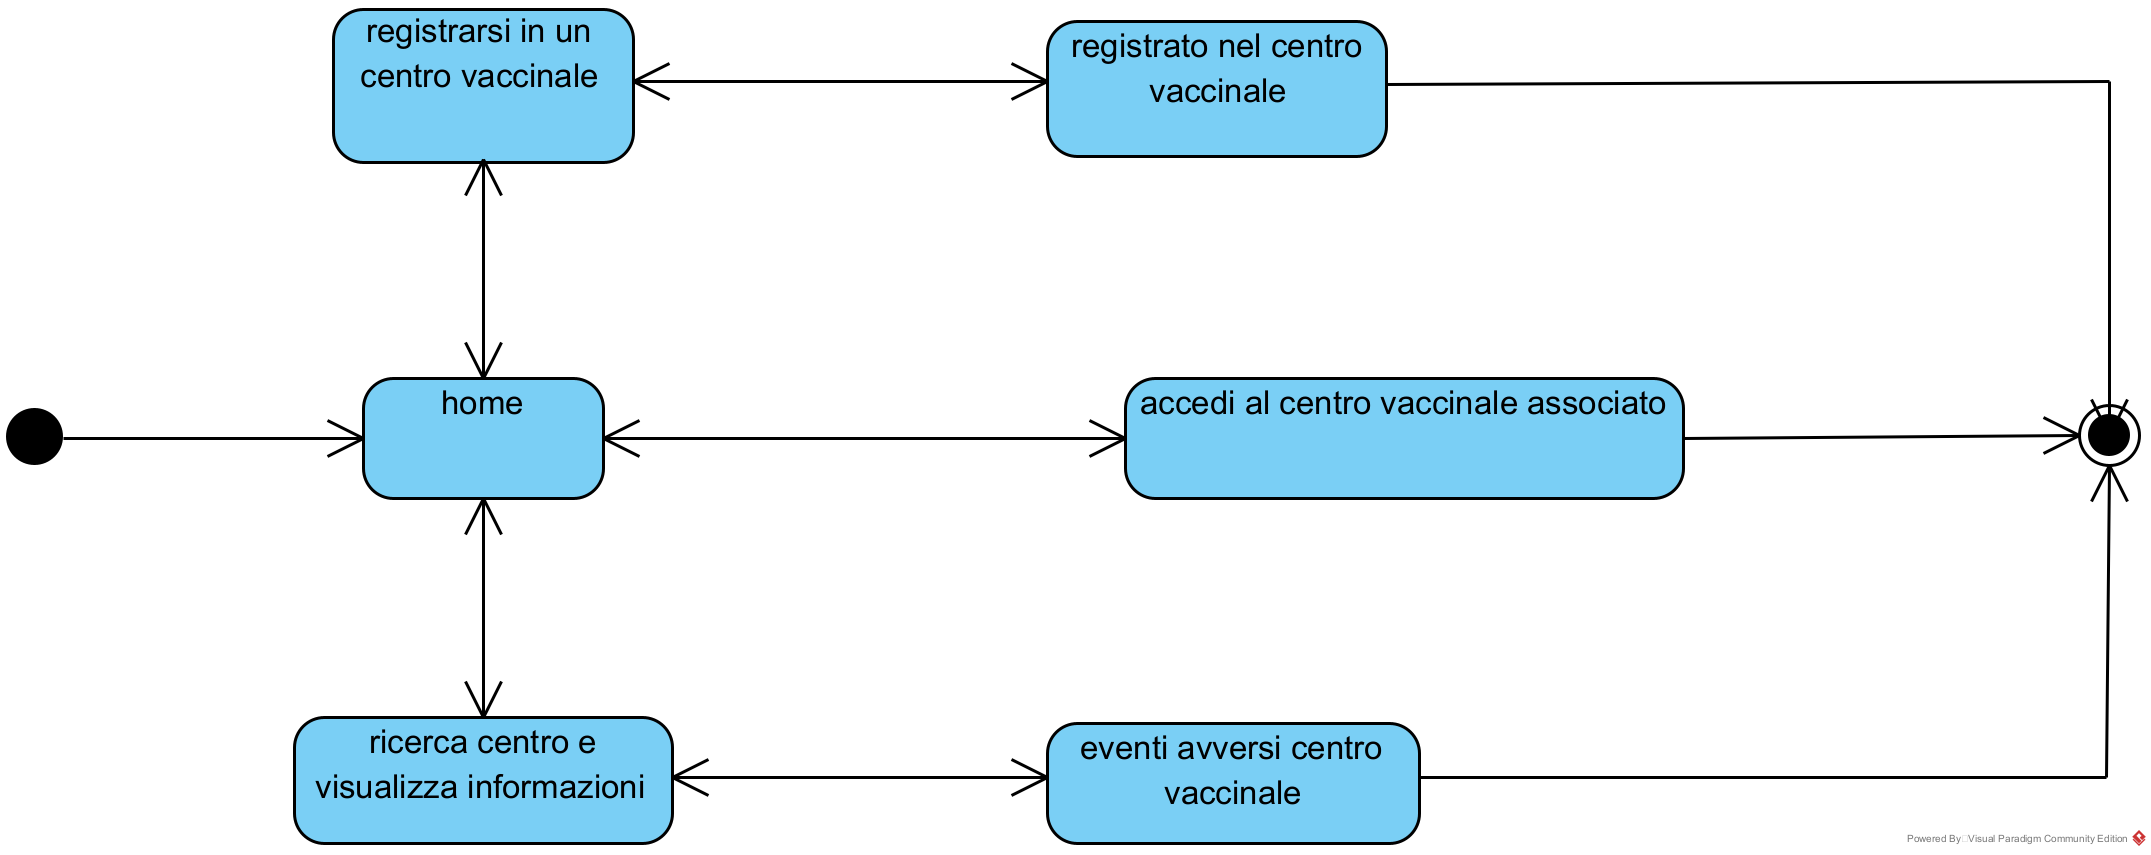
\includegraphics[width=\textwidth]{./img/StateMachineDiagramCittadini}
	\caption{State diagram del modulo cittadino}
\end{figure}

\begin{figure}[t]
	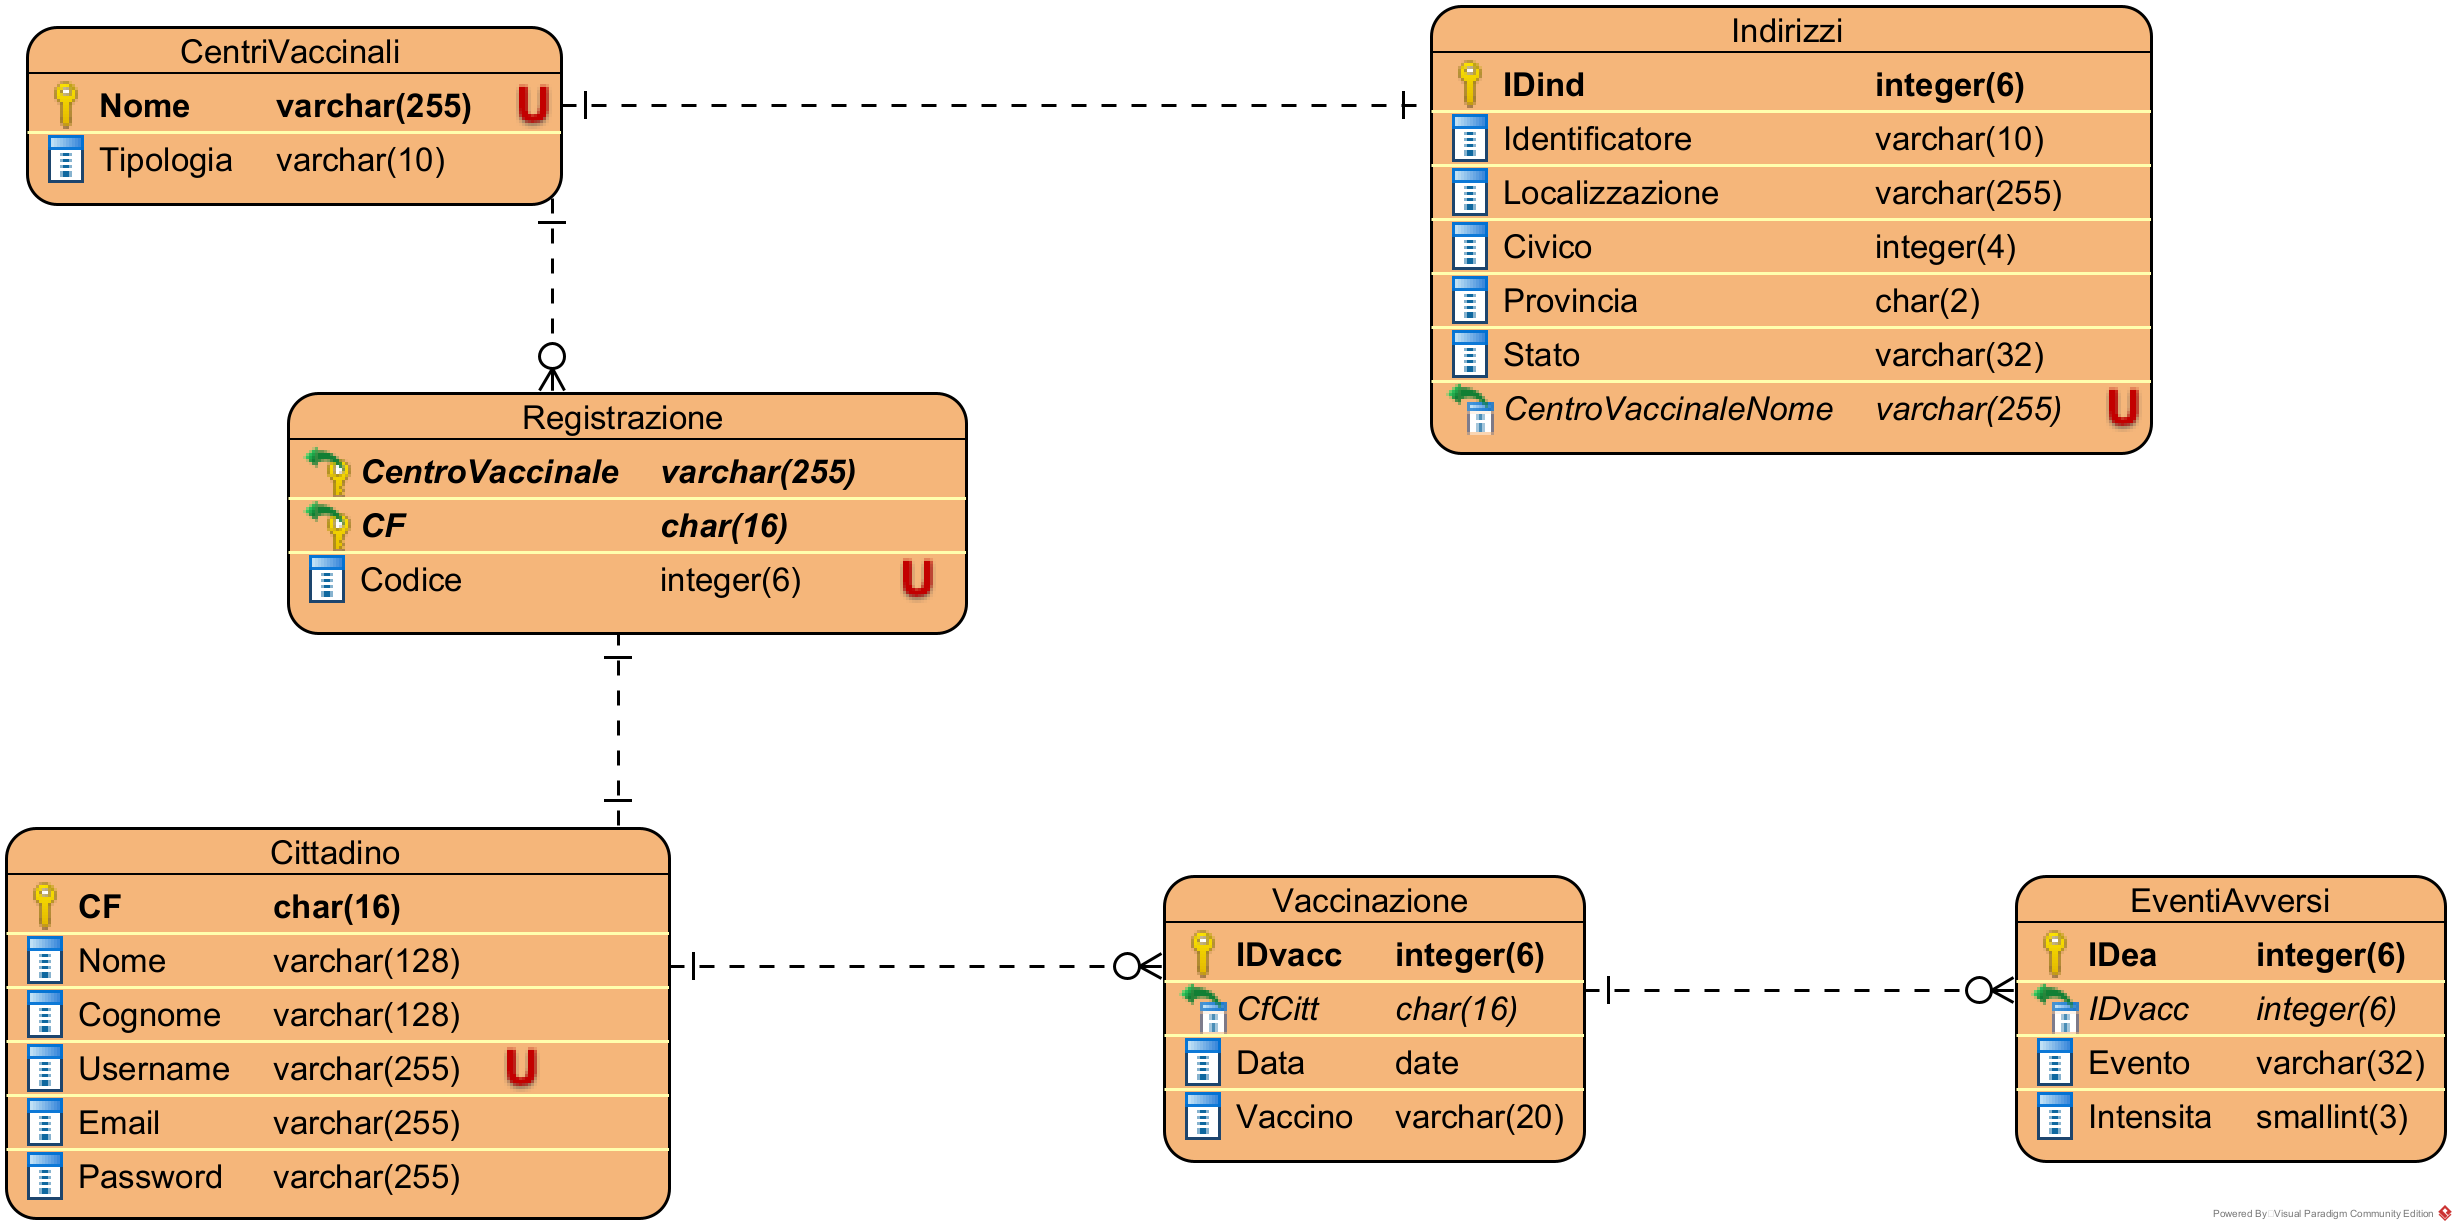
\includegraphics[width=\textwidth]{./img/CentriVaccinaliDB}
	\caption{Diagramma entità-relazione del database}
\end{figure}